\documentclass[22pt]{beamer}
\usepackage[orientation=portrait, size=custom, width=91.44, height=91.44,scale=1.2]{beamerposter} % 36in*2.5 = 90cm
\usepackage[absolute,overlay]{textpos}
\usepackage{bookmark} %pdflatex says to use this to avoid errors...
\usepackage{graphicx} %for including images
\graphicspath{{figs/}} %location of images
\usepackage{wrapfig} %wrap text around the images
\usepackage{lipsum} %wrap text around the images
\usepackage{listingsutf8}    %package for code environment; use this instead of verbatim to get automatic line break; use this instead of listings to get (•)
\usepackage{amsmath}
\usepackage{gensymb}
\usepackage[export]{adjustbox}
\usepackage[skins,theorems]{tcolorbox}
\usepackage{tikz}
\newcommand*\circled[1]{\tikz[baseline=(char.base)]{
            \node[shape=circle,draw,inner sep=2pt] (char) {#1};}}
\usepackage{array}
\usepackage{booktabs,adjustbox}
\usepackage{subcaption} 

%\mode<presentation>
%this doesn't seem to make any difference; leave for now for trying out
\usetheme{Berlin}
\definecolor{MacBlue}{rgb}{0.10196,0.22353,0.53725}
\definecolor{MacMaroon} {rgb}{0.47843, 0, 0.23137}
\definecolor{MacMaroon2} {rgb}{0.47451, 0, 0}
\definecolor{MacGray}{rgb}{0.50196,0.49804,0.51765}
\definecolor{MacMaroon3}{rgb}{00.47,0.2,0.31}
\definecolor{MacGold}{rgb}{1, 0.75,0.35}
\usecolortheme[named=MacMaroon2]{structure}
\setbeamertemplate{caption}[numbered]
\setbeamertemplate{navigation symbols}{}

\title{Applying TensorFlow Machine Learning and Crowd Sourced Data to Better Understand Campus Environments: Pinpointr}
\subtitle{}  %probably want a better subtitle
  \author[Kipp, McKay, Ronald, Timpau, Deluca \& Anand]{Matthew Kipp, Sean McKay, Brandon Ronald, Victor Timpau, supervised by Dr.~Patrick Deluca and Dr.~Christopher Anand$^\dagger$ \vspace{0.3cm} \newline \small \{kippmr, mckaysm, timpauv, delucapf, anandc\}@mcmaster.ca}
  \institute[McMaster University]{$^\dagger$Department of Computing and Software, McMaster University

1280 Main St. W, Hamilton, Ontario, Canada L8S 4L8}
  \date{December 5, 2018}

\begin{document}
%compile with pdflatex

%there is only one frame, because there is only one page; yeah, it's a poster
%textblock and block seem to work nicely to organize layout
\begin{frame}[fragile]

\begin{textblock}{2}(0.7,1)

\includegraphics[height=8.5cm]{englogo.png}
\end{textblock}

\begin{textblock}{2}(12.7,0.80)

\includegraphics[height=10.5cm]{fireball-logo.png} 
\end{textblock}

\begin{textblock}{8}(4,1)
\titlepage
\end{textblock}

\begin{textblock}{7}(4.25,3.1)
\begin{figure}[htbp] %  figure placement: here, top, bottom, or page
 \centering
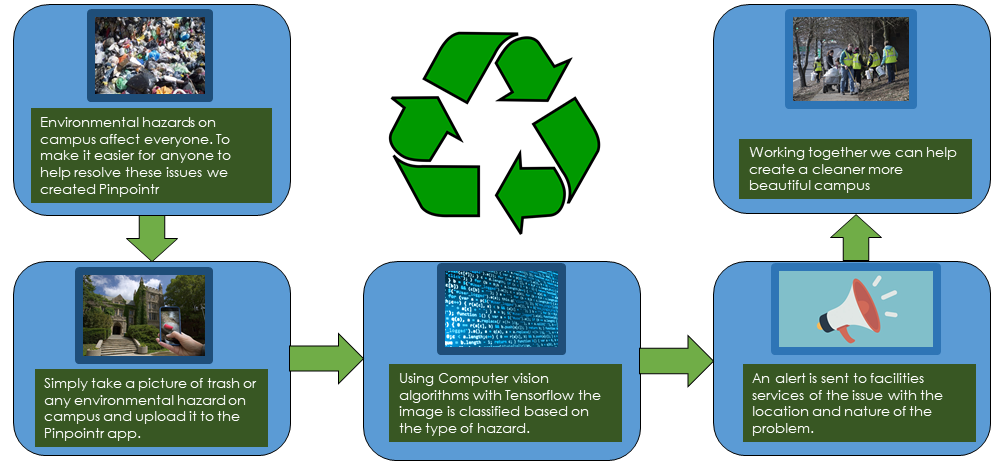
\includegraphics[height=20cm]{flowchart.png}
\end{figure}
\end{textblock}

\begin{textblock}{3.5}(0.5, 3.1)
\begin{block}{Problem: Waste on Campus}
Over 2000 Metric tonnes of waste was generated on campus in 2017 \cite{mcmasterwaste}. To reduce the amount of waste disposed of improperly it’s important to have everyone on campus participate. \par

Issues from full garbage cans to broken water fountains can increase the amount of waste generated. \par

To make reporting any environmental hazards or facilities issues on campus easier, we created Pinpointr, an integrated solution for managing waste on campus. 
\end{block}

\begin{block}{Solution: Pinpointr}
Pinpointr is an app that allows anyone to document an issue on campus with a single photo and a button press. \par
The app uses machine learning technology and geolocation to figure out where and what the issue is. From there, it sends an alert to facilities services, so they can create a work order to deal with the issue. \par
 It also includes the ability to scan QR codes placed on facilities around campus, in order to report issues with specific trash cans, water fountains, etc.
\end{block}


%Could probably cut this down quite a bit
\begin{block}{User Adoption Strategy}
Phase 1 (January 2019)
\begin{itemize}
\item Beta version of app with basic functionality (Upload and Classify photos, display location on map)
\item Small team of testers to determine the ease of use of the app, identify bugs on the users side
\end{itemize}
Phase 2 (February 2019)
\begin{itemize}
\item Revised Pinpointr app including QR code recognition 
\item Place QR codes on facilities that may need servicing (Trash bins, water fountains)
\item A small team of custodial staff testing the software to see if it makes their work easier and more efficient, identify bugs on the staff side
\end{itemize}
Phase 3 (Late February)
\begin{itemize}
\item Multiple platforms for sending pictures (Text, Twitter, App)
\item Greater adoption by custodial staff
\end{itemize}
Phase 4 (March 2019)
\begin{itemize}
\item Promotion, incentives for downloading the app and reporting environmental hazards
\item Use derived metrics from the app to inform and improve purchasing decisions for other staff on campus
\end{itemize}
\end{block}

\end{textblock}

\begin{textblock}{3.5}(12, 3.1)
\begin{block}{Overall Goals}
\begin{itemize}
\item Decrease response time for dealing with environmental hazards and broken facilities
\item Identify problem areas around campus, so steps can be taken to add more waste disposal options
\item Identify common sources of waste that originate on campus, so steps can be taken to reduce unnecessary packaging or transition to more environmentally friendly options
\item Reduce the amount of waste on campus by having users participate in keeping the campus clean
\end{itemize}
\end{block}

\begin{block}{Other Tools}
Tools to help display hazards and their location on the Pinpointr website
\begin{itemize}
\item ArcGIS and Leaflet to place points on map, categorize points in sections of campus or by buildings
\item ESRI to provide a ArcGIS javascript API for applying location-based analytics and loading results to the web
\item Leaflet to provide an open-source javascript library for mobile-friendly interactive maps
\end{itemize}
\end{block}

\begin{block}{Improvements on Existing Software}
Litterati is an app with a similar purpose. It tracks litter collected by its users on a map, using user submitted tags to group litter based on the brand and material. The collected data has been used succesfully to justify changes in environmental policy at parks and purchasing decisions at schools \cite{litterati}. /par
To improve and differentiate our software, we use computer vision to classify the litter rather than relying on user submitted tags. We also integrate alerts into our map feature, allowing us to work directly with custodial staff to clean up our campus.
\end{block}

\begin{block}{References}
\setbeamertemplate{bibliography item}{\insertbiblabel}
\bibliographystyle{ieeetr}
{\scriptsize
\bibliography{bib}}
\end{block}

\begin{figure}[htbp]
\centering

\includegraphics[height=5cm]{googlebrain-logo.png}
\hspace{1cm}

\includegraphics[height=5cm]{tensorflow-logo.png}
\hspace{1cm}

\includegraphics[height=5cm]{python-logo.png}
\hspace{1cm}

\includegraphics[height=5cm]{esri-logo.png}
\end{figure}

\end{textblock}

\begin{textblock}{7.25}(0.5,7.1)



\end{textblock}



\begin{textblock}{7.25}(4.375,7.1)
\begin{block}{Image Classification And Object Recognition with TensorFlow}
TensorFlow
\begin{itemize}
\item Built by GoogleBrain, combines several machine-learning models and algorithms into an open-source library.
\end{itemize}
MobileNets Via TensorFlow Lite
\begin{itemize}
\item TensorFlow Lite models such as MobileNets provide low-latency, lightweight TensorFlow solution for mobile devices.
\item On-device machine learning inference.
\item Model-training methodology based on convolutional neural network architecture.
\end{itemize}
\begin{figure}[htbp] %  figure placement: here, top, bottom, or page
\begin{subfigure}{0.95\textwidth}
   \centering
   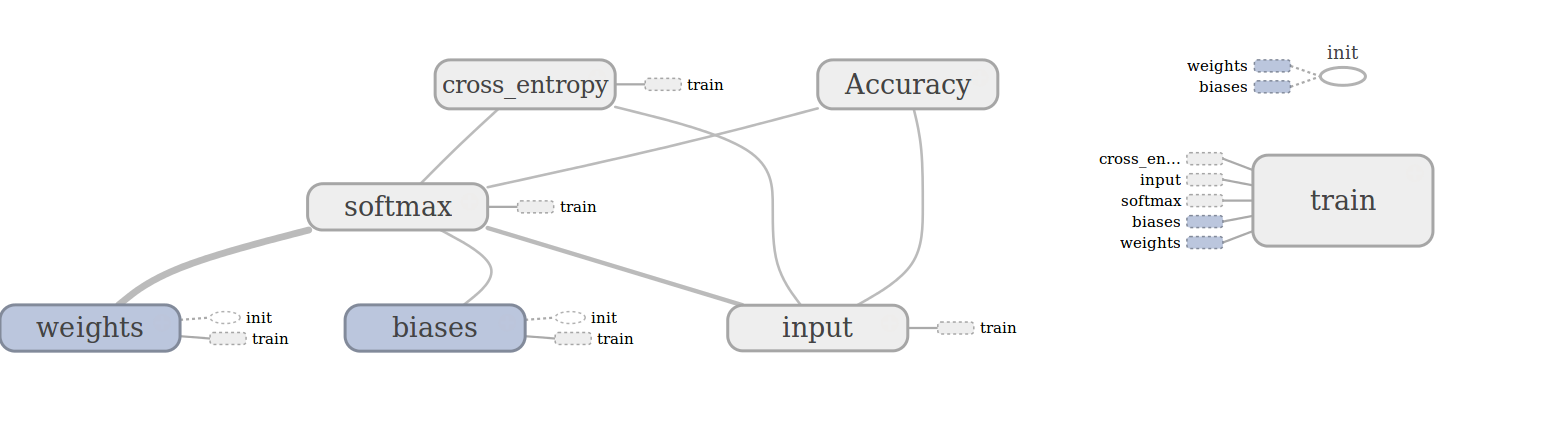
\includegraphics[height=10cm]{softmax.png}
   \caption*{\textit{Figure 1:} “softmax” represents the final output layer, providing the final object categorization and probability. The bottleneck nodes to the right represent a series of layers created during the training process.}
   \label{fig:softmax}
\end{subfigure}
\end{figure}
TensorBoard
\begin{itemize}
\item Data visualization platform for model training analysis.
\item Continuous monitoring of model accuracy.
\end{itemize}
\begin{figure}[htbp] %  figure placement: here, top, bottom, or page
\begin{subfigure}{0.95\textwidth}
   \centering
   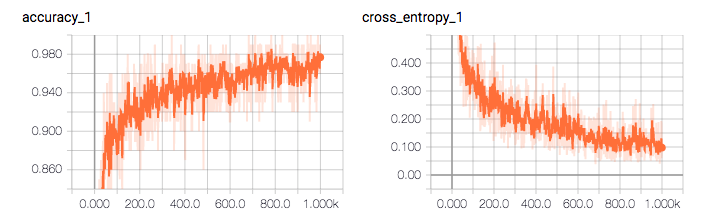
\includegraphics[height=10cm]{interface.png}
   \caption*{\textit{Figure 2:} Tensorboard Interface:  As the training dataset grows and the number of training sessions increases, the accuracy of the model approaches 1, while cross entropy approaches 0.}
   \label{fig:interface}
\end{subfigure}
\end{figure}
\end{block}
\end{textblock}


\end{frame}
\end{document}
